\section{Activity \# 2 - Like in Ski}


\frameboxbegin{Summary of the Activity}
Total duration: 30 minutes
The required equipment for this activities should be:
\begin{itemize}
\item 1 robot POB,
\item 1 computer with Risbee software installed,
\item 1 mini-USB cable,
\item 2 objects/targets,
\item the booklet ``Quick Start Risbee''.
\end{itemize}
\frameboxend

\frameboxbegin{Motion - 5 minutes}
\begin{description}
\item[Objective:] To be able to move forward the robot.
\item[I am learning:] \hfill \\ \vspace{-4ex}
  \begin{itemize}
  \item To order the icons in order to make a simple program,
  \item To move the robot forward,
  \item The concept of trajectory.
  \end{itemize}
\end{description}
\frameboxend

\frameboxbegin{Slalom - 20 minutes}
\begin{flushleft}
\begin{description}
\item[Objectives:] To move the robot from a landmark ``A'' to a landmark ``C'' passing by a landmark ``B'' by bending as depicted in Fig.\,\ref{fig:s2}. The player can chose either to stop at each landmark after each bend or to travel in one shot.
\begin{minipage}[c]{\textwidth}
\centering
\tikzstyle{target}=[circle,thick,minimum size=2cm,draw=blue!80,fill=blue!20]
\vspace{1ex}
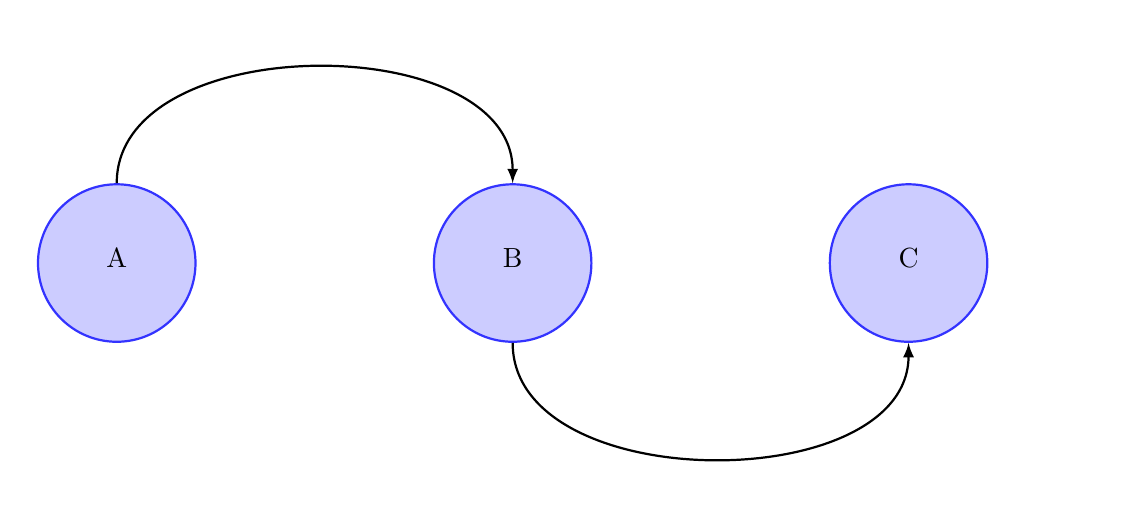
\begin{tikzpicture}[>=latex,text height=1ex,text depth=0.25ex]
  \matrix[row sep=1cm,column sep=1.5cm] {
    \node (A) [target] {A}; &
    &
    \node (B) [target] {B}; &
    &
    \node (C) [target] {C}; &
    \\
  };
  \path[->]
  (A) edge[bend left=90,thick] (B)
  (B) edge[bend right=90,thick] (C);
\end{tikzpicture}
\captionof{figure}{Landmarks positioning.}\label{fig:s2}
\end{minipage}
\item[I am learning:] \hfill \\ \vspace{-1ex}
  \begin{itemize}
  \item To discover some additional icons,
  \item To move the robot until a given landmark,
  \item The concept of trajectory,
  \item The concept of angle,
  \item The change of direction.
  \end{itemize}
\end{description}
\end{flushleft}
\frameboxend

\frameboxbegin{Race - 5 minutes}
\begin{flushleft}
\begin{description}
\item[Objective:] To make a race between two robots. Move the position of the landmark ``B'' and ``C'' which will have to be reached by the players.
\item[I am learning:] \hfill \\ \vspace{-1ex}
  \begin{itemize}
  \item To discover some additional icons,
  \item To control the speed of the engines,
  \item To challenge other players.
  \end{itemize}
\end{description}
\end{flushleft}
\frameboxend
